\documentclass[11pt,a4paper,twocolumn]{article}
\usepackage[utf8]{inputenc}
\usepackage[french]{babel}
\usepackage[T1]{fontenc}
\usepackage{lmodern}
\usepackage{amsmath}
\usepackage{amsfonts}
\usepackage{amssymb}
\usepackage{graphicx}
\usepackage{booktabs}
\usepackage{array}
\usepackage{geometry}
\usepackage{xcolor}
\usepackage{hyperref}
\usepackage{cite}
\usepackage{listings}
\usepackage{microtype}
\usepackage[font=small,labelfont=bf]{caption}
\usepackage{titlesec}
\usepackage{tikz}
\usetikzlibrary{arrows.meta}

\geometry{top=2.0cm, bottom=2.0cm, left=1.8cm, right=1.8cm}
\graphicspath{{plots/}}

% ---- Charte graphique ----
\definecolor{accent}{RGB}{15,82,140}      % bleu profond pour titres
\definecolor{accentlight}{RGB}{230,238,246}

\hypersetup{colorlinks=true, linkcolor=accent, citecolor=accent, urlcolor=accent}

% Titres de section colorés avec filet
\titleformat{\section}{\normalfont\large\bfseries\color{accent}}{\thesection}{0.6em}{}[{\color{accent!30}\titlerule[0.8pt]}]
\titleformat{\subsection}{\normalfont\normalsize\bfseries\color{accent!85!black}}{\thesubsection}{0.5em}{}
\titlespacing*{\section}{0pt}{1.4ex plus 1ex minus .2ex}{1ex}

% Espacement des lignes légèrement aéré pour la lisibilité
\renewcommand{\arraystretch}{1.15}

\title{\textbf{Vérification, validation et estimation de la longueur effective d'un résonateur de Helmholtz par un solveur de différences finies axisymétrique} \\ \large Étude de convergence GCI, comparaison à des mesures publiées et modèle réduit des pertes}
\author{\textbf{Projet de Recherche Acoustique Numérique}}
\date{\today}

\begin{document}

\maketitle

\begin{abstract}
Ce travail présente la vérification, la validation et l'exploitation d'un solveur de différences finies (FDM) fréquentiel pour l'équation de Helmholtz en coordonnées cylindriques axisymétriques $(r,z)$, appliqué à un résonateur de Helmholtz ; la singularité sur l'axe de symétrie est levée par la règle de L'Hôpital. Le \emph{code} est vérifié par solution manufacturée (ordre de convergence $2{,}03$ sur domaine lisse). La \emph{solution} est vérifiée par une étude GCI de Roache sur trois grilles ($h \in \{2, 1, 0{,}5\}\text{ mm}$, cinq longueurs de col), complétée d'une quatrième grille de contrôle ($0{,}25$ mm) confirmant la stabilité de l'ordre observé ($\approx 0{,}9$–$1{,}1$, dégradé par la géométrie en escalier) et des extrapolations de Richardson ; l'incertitude numérique est d'environ $2\%$. Le \emph{modèle} fait l'objet d'une première validation sur deux configurations expérimentales publiées (Selamet \emph{et al.}), reproduites à $0{,}6\%$ et $2{,}2\%$ sans paramètre ajusté. La loi d'échelle $f_0(L)$ est ensuite analysée sur les fréquences extrapolées, en propageant l'incertitude numérique traitée comme intervalle indicatif (le GCI n'étant pas un écart-type statistique) : une loi de puissance empirique et le modèle physique à longueur effective, $f_0 = A_H/\sqrt{L + \Delta L_{\mathrm{eff}}}$, sont statistiquement indiscernables ($\Delta\text{AICc} = 0{,}3$ à $1{,}8$ selon l'échantillon, $5$ à $12$ longueurs), mais le modèle physique est préféré : $A_H = 47{,}7 \pm 1{,}4$ compatible avec la valeur théorique $48{,}25$, $\Delta L_{\mathrm{eff}} \approx 0{,}66$–$0{,}68\,R_{col}$ comparable à la correction de Rayleigh/Ingard, et prédiction leave-one-out dix fois meilleure. Une configuration à impédance de rayonnement de piston bafflé décompose cette correction (intérieure $0{,}68\,R_{col}$ ; décalage $0{,}825\,R_{col}$, cohérent à $2{,}8\%$ avec la réactance imposée $8R_{col}/(3\pi)$ — test de cohérence, non calcul \emph{ab initio}). Enfin, un modèle réduit d'amortissement calibré sur l'estimation viscothermique de couche limite ($Q\approx47$) illustre les signatures des pertes sans les résoudre.

\vspace{0.5em}
\noindent\textbf{Mots-clés :} résonateur de Helmholtz ; différences finies axisymétriques ; vérification et validation ; solution manufacturée ; indice de convergence de maillage (GCI) ; longueur effective ; correction de bout ; pertes viscothermiques.
\end{abstract}

\vspace{0.4em}
\begingroup
\setcounter{tocdepth}{1}
\renewcommand{\contentsname}{\normalsize\color{accent}\textbf{Sommaire}}
{\small\tableofcontents}
\endgroup
\vspace{0.4em}
\hrule
\vspace{0.8em}

\section{Introduction et Théorie Classique}
Le résonateur de Helmholtz est un système acoustique fondamental \cite{helmholtz1860} constitué d'un col (longueur $L$, section $S_{col}$) connecté à une cavité rigide de grand volume $V_{cav}$. Sous l'excitation d'une perturbation extérieure, la colonne d'air du col oscille comme un piston rigide (effet de masse inertielle), comprimant l'air de la cavité qui agit comme un ressort pneumatique.

Dans l'approximation classique monodimensionnelle et sans pertes, la fréquence propre de résonance $f_0$ est donnée par la formule d'oscillation libre :
\begin{equation}
\label{eq:helmholtz_1d_pure}
f_0 = \frac{c}{2\pi} \sqrt{\frac{S_{col}}{V_{cav} L}}
\end{equation}
où $c \approx 343\text{ m/s}$ désigne la vitesse du son. Pour un col cylindrique de rayon $R_{col}$ et une cavité cylindrique de rayon $R_{cav}$ et de hauteur $H_{cav}$, le modèle théorique pur s'exprime sous la forme d'une loi de puissance en $L^{-0{,}5}$ :
\begin{equation}
f_0 = \frac{c}{2\pi} \frac{R_{col}}{R_{cav}} \frac{1}{\sqrt{H_{cav} L}} = \frac{A_H^{\mathrm{th}}}{\sqrt{L}}
\end{equation}
Pour notre géométrie de référence ($R_{col}=1\text{ cm}$, $R_{cav}=4\text{ cm}$, $H_{cav}=8\text{ cm}$), la constante théorique vaut $A_H^{\mathrm{th}} \approx 48{,}25\text{ m}^{1/2}/\text{s}$. (La constante du modèle de fréquence est notée $A_H$ dans tout l'article, le symbole $R_{col}$ étant réservé au rayon du col, afin d'éviter toute collision de notation.)

Cependant, cette théorie 1D repose sur l'hypothèse d'ondes planes parfaites. Elle néglige la distorsion bidimensionnelle du champ acoustique aux extrémités du col, forçant l'introduction empirique d'une correction de bout $\Delta L$ \cite{rayleigh1896, peters2003end} :
\begin{equation}
\label{eq:helmholtz_correction}
f_0(L) = \frac{c}{2\pi} \sqrt{\frac{S_{col}}{V_{cav} (L + \Delta L)}} = \frac{A_H^{\mathrm{th}}}{\sqrt{L + \Delta L}}
\end{equation}
où $\Delta L$ est supposée constante pour une géométrie de col donnée (de l'ordre de $0{,}6 \, R_{col}$ à $0{,}85 \, R_{col}$). Ce travail explore dans quelle mesure un solveur physique FDM s'écarte de ce modèle à correction constante en faisant varier la longueur du col $L$, et confronte ses résultats aux valeurs de référence de la littérature.

\section{Développement du Solveur FDM}
\subsection{Formulation Fréquentielle et Traitement de la Singularité}
Sous excitation harmonique établie de pulsation $\omega = 2\pi f$, la pression complexe $p(r,z)$ satisfait l'équation de Helmholtz en coordonnées cylindriques axisymétriques ($\partial p/\partial \theta = 0$) :
\begin{equation}
\label{eq:helmholtz_radial}
\frac{\partial^2 p}{\partial r^2} + \frac{1}{r}\frac{\partial p}{\partial r} + \frac{\partial^2 p}{\partial z^2} + k^2 p = 0
\end{equation}
où $k = \omega/c$ désigne le nombre d'onde.

Le terme radial $\frac{1}{r}\frac{\partial p}{\partial r}$ pose une singularité indéterminée sur l'axe de révolution $r=0$. En appliquant la règle de L'Hôpital pour $r \to 0$, nous avons :
\begin{equation}
\lim_{r \to 0} \frac{1}{r}\frac{\partial p}{\partial r} = \lim_{r \to 0} \frac{\frac{\partial}{\partial r}\left(\frac{\partial p}{\partial r}\right)}{\frac{\partial}{\partial r}(r)} = \frac{\partial^2 p}{\partial r^2}
\end{equation}
Sur l'axe de symétrie ($r=0$), l'équation de Helmholtz axisymétrique se simplifie sous forme régulière :
\begin{equation}
\label{eq:lhopital_axis}
2\frac{\partial^2 p}{\partial r^2} + \frac{\partial^2 p}{\partial z^2} + k^2 p = 0 \quad (\text{avec } \frac{\partial p}{\partial r} = 0)
\end{equation}

Les conditions aux limites appliquées sur la grille structurée uniforme du plan méridien $(r,z)$ (pas spatial $h$) sont :
\begin{itemize}
    \item \textbf{Source d'excitation} (inlet) à $z=0$, $r \in [0, R_{col}]$ : Condition de Dirichlet $p(r,0) = p_0 = 1\text{ Pa}$.
    \item \textbf{Axe de symétrie} ($r=0$) : Condition de symétrie Neumann homogène $\frac{\partial p}{\partial r} = 0$, résolue par le stencil régularisé \eqref{eq:lhopital_axis}.
    \item \textbf{Parois rigides} : Condition de flux nul Neumann homogène $\frac{\partial p}{\partial n} = 0$ implémentée par nœuds virtuels solides ($p_{\mathrm{solide}} = p_{\mathrm{fluide}}$).
\end{itemize}

La Figure \ref{fig:fdm_grid_nodes} illustre schématiquement le maillage et la classification des nœuds sur le domaine fluide du résonateur.

\begin{figure}[ht]
\centering
\begin{tikzpicture}[scale=0.75]
    \draw[step=0.5cm, gray!20, very thin] (-0.5,-0.5) grid (5.5,4.5);
    \draw[-{Stealth}, thick] (0,-0.5) -- (0,4.8) node[above] {$z$ (axe)};
    \draw[-{Stealth}, thick] (-0.5,0) -- (5.8,0) node[right] {$r$};

    % Inlet Dirichlet
    \foreach \x in {0, 0.5, 1.0} {
        \node[circle, fill=red, inner sep=1.8pt] at (\x, 0) {};
    }
    \node[red, right] at (1.2,0.2) {\small Inlet ($p=p_0$)};

    % Axe Neumann
    \foreach \y in {0.5, 1.0, 1.5, 2.0, 2.5, 3.0, 3.5, 4.0} {
        \node[circle, fill=blue, inner sep=1.8pt] at (0, \y) {};
    }
    \node[blue, left] at (-0.1, 2.0) {\small Axe $r=0$};

    % Solid boundary
    \foreach \y in {0.5, 1.0, 1.5} {
        \node[circle, fill=black!70, inner sep=1.8pt] at (1.0, \y) {};
    }
    \foreach \x in {1.0, 1.5, 2.0, 2.5, 3.0, 3.5, 4.0} {
        \node[circle, fill=black!70, inner sep=1.8pt] at (\x, 1.5) {};
    }
    \foreach \y in {2.0, 2.5, 3.0, 3.5, 4.0} {
        \node[circle, fill=black!70, inner sep=1.8pt] at (4.0, \y) {};
    }
    \node[black!70, right] at (4.1, 3.0) {\small Parois solides};

    % Fluid nodes
    \foreach \x in {0.5} {
        \foreach \y in {0.5, 1.0} {
            \node[circle, fill=green!60!black, inner sep=1.8pt] at (\x, \y) {};
        }
    }
    \foreach \x in {0.5, 1.0, 1.5, 2.0, 2.5, 3.0, 3.5} {
        \foreach \y in {2.0, 2.5, 3.0, 3.5, 4.0} {
            \node[circle, fill=green!60!black, inner sep=1.8pt] at (\x, \y) {};
        }
    }
    \node[green!60!black, fill=white, inner sep=1pt] (lblfluid) at (2.6, 5.15) {\small Nœuds fluides};
    \draw[green!60!black, -{Stealth}, thin] (lblfluid) -- (2.0, 4.1);
\end{tikzpicture}
\caption{Classification géométrique des nœuds et conditions aux limites sur le domaine FDM axisymétrique.}
\label{fig:fdm_grid_nodes}
\end{figure}

\section{Étude de Convergence en Maillage}
\label{sec:convergence}
Pour quantifier l'erreur de discrétisation spatiale, nous résolvons la fréquence propre $f_0$ sur trois grilles de pas spatial décroissant à ratio constant ($h \in \{2, 1, 0{,}5\}\text{ mm}$, ratio de raffinement $r = 2$) pour les cinq longueurs de col de l'étude, $L \in \{2, 3, 4, 5, 6\}\text{ cm}$. Les résultats sont récapitulés dans le Tableau \ref{tab:mesh_sensitivity}.

\begin{table*}[t]
\centering
\caption{Fréquences propres $f_0$ (Hz) du solveur FDM sur les trois grilles de raffinement}
\label{tab:mesh_sensitivity}
\begin{tabular}{c*{6}{>{\centering\arraybackslash}p{1.8cm}}}
\toprule
L (cm) & \multicolumn{2}{c}{$h = 2\text{ mm}$} & \multicolumn{2}{c}{$h = 1\text{ mm}$} & \multicolumn{2}{c}{$h = 0{,}5\text{ mm}$} \\
\cmidrule(r){2-3} \cmidrule(lr){4-5} \cmidrule(l){6-7}
 & $f_0$ (Hz) & Nœuds & $f_0$ (Hz) & Nœuds & $f_0$ (Hz) & Nœuds \\
\midrule
2{,}0 & 309{,}8 & 1\,071 & 301{,}4 & 4\,141 & 297{,}0 & 16\,281 \\
3{,}0 & 264{,}6 & 1\,176 & 257{,}4 & 4\,551 & 253{,}7 & 17\,901 \\
4{,}0 & 234{,}6 & 1\,281 & 228{,}2 & 4\,961 & 224{,}8 & 19\,521 \\
5{,}0 & 212{,}8 & 1\,386 & 207{,}0 & 5\,371 & 203{,}9 & 21\,141 \\
6{,}0 & 196{,}0 & 1\,491 & 190{,}7 & 5\,781 & 188{,}0 & 22\,761 \\
\bottomrule
\end{tabular}
\end{table*}

Nous observons une baisse systématique de la fréquence propre lors du raffinement de la grille, compatible avec une meilleure représentation de la transition col–cavité et de la masse acoustique effective. Pour quantifier l'erreur de discrétisation de manière objective, nous appliquons la méthodologie de Roache fondée sur l'indice de convergence de maillage (\emph{Grid Convergence Index}, GCI) \cite{roache1994perspective}. À partir des fréquences sur les trois grilles ($f_1$ fine, $f_2$ intermédiaire, $f_3$ grossière), l'ordre de convergence observé $p$, l'extrapolation de Richardson $f_{h\to0}$ et l'incertitude numérique GCI de la grille fine s'écrivent :
\begin{align}
p &= \frac{\ln\left(|f_3 - f_2|/|f_2 - f_1|\right)}{\ln r}, \quad
f_{h\to0} = f_1 + \frac{f_1 - f_2}{r^p - 1} \\
\mathrm{GCI}_{\mathrm{fin}} &= F_s\,\frac{|(f_2 - f_1)/f_1|}{r^p - 1}, \quad F_s = 1{,}25
\end{align}
Les résultats sont consignés dans le Tableau \ref{tab:gci}.

\begin{table}[h]
\centering
\caption{Convergence de maillage : ordre observé $p$, extrapolation de Richardson et incertitude GCI sur la grille fine}
\label{tab:gci}
\begin{tabular}{ccccc}
\toprule
$L$ (cm) & $f_{0,\,\mathrm{fin}}$ (Hz) & $p$ & $f_{h\to0}$ (Hz) & GCI (\%) \\
\midrule
2{,}0 & 297{,}0 & 0{,}93 & 292{,}2 & 2{,}04 \\
3{,}0 & 253{,}7 & 0{,}95 & 249{,}7 & 1{,}97 \\
4{,}0 & 224{,}8 & 0{,}91 & 221{,}0 & 2{,}14 \\
5{,}0 & 203{,}9 & 0{,}90 & 200{,}3 & 2{,}20 \\
6{,}0 & 188{,}0 & 0{,}93 & 184{,}9 & 2{,}05 \\
\bottomrule
\end{tabular}
\end{table}

L'ordre de convergence observé, $p \approx 0{,}92$, est proche de $1$ : bien que le stencil intérieur soit formellement d'ordre $2$, la représentation en escalier des parois et du raccordement col–cavité dégrade la convergence vers le premier ordre. L'incertitude numérique sur la grille la plus fine est de l'ordre de $2\%$. L'extrapolation de Richardson fournit une estimation de référence utilisée dans la suite ; sa fiabilité suppose toutefois un régime proche de l'asymptotique, hypothèse contrôlée comme suit.

\paragraph{Contrôle du régime asymptotique (quatrième grille).} Une grille supplémentaire $h=0{,}25$ mm est calculée pour $L=2$ et $4$ cm (jusqu'à $77\,441$ nœuds), donnant deux triplets de raffinement par longueur. L'ordre observé reste stable ($p = 0{,}933 \to 0{,}936$ pour $L=2$ cm ; $0{,}914 \to 1{,}06$ pour $L=4$ cm) et les extrapolations de Richardson des deux triplets coïncident à $0{,}01\%$ et $0{,}32\%$ respectivement — très en deçà du GCI —, tandis que le GCI de la grille la plus fine descend à environ $1\%$. Les références extrapolées utilisées dans la suite sont donc stables au niveau de précision requis, sans que l'indépendance asymptotique stricte soit revendiquée.

Il convient de distinguer cette \emph{vérification de solution} (ordre $\approx 1$, limité par la géométrie) de la \emph{vérification du code} \cite{roache1998verification}. Cette dernière est établie par une solution manufacturée (MMS) : sur un domaine rectangulaire lisse (sans escalier), une solution analytique régulière sur l'axe est imposée via un terme source, et l'erreur $L_2$ décroît à l'\textbf{ordre $2{,}03$} sur quatre grilles ($h \in \{4, 2, 1, 0{,}5\}$ mm), confirmant que le stencil axisymétrique est bien d'ordre $2$. La perte d'un ordre sur le résonateur réel est donc principalement imputable à la discrétisation en escalier de la géométrie — sans exclure des contributions secondaires (traitement des coins et des conditions de Neumann, extraction du pic) — et non à une erreur de programmation.

\section{Première Validation sur Deux Configurations Expérimentales Publiées}
\label{sec:validation}
La vérification (du code par MMS, de la solution par GCI) ne dit rien de l'adéquation du modèle à la réalité physique : c'est le rôle de la \emph{validation}. À défaut d'une campagne expérimentale propre, le solveur est confronté aux mesures publiées de Selamet \emph{et al.} \cite{selamet1997circular}, dont la configuration — col cylindrique débouchant dans une cavité cylindrique coaxiale — est exactement celle du présent modèle axisymétrique : col $d_c = 4{,}044$ cm, $l_c = 8{,}5$ cm, volume fixe $V = 4500\text{ cm}^3$, rapport longueur/diamètre de cavité $l/d$ variable. Les fréquences de résonance y sont mesurées en tube d'impédance (pic de perte par transmission) et confirmées par une méthode d'éléments de frontière 3-D avec un écart d'à peine 1 Hz.

À la résonance d'une branche latérale, l'impédance d'entrée du col s'annule ($p\approx0$ à l'embouchure) : la condition de Dirichlet du solveur est donc la représentation adéquate de cette configuration, d'autant que le col occupe $83\%$ du diamètre du tube (correction de bout côté tube marginale). Le Tableau \ref{tab:selamet} compare les fréquences propres calculées, sans aucun paramètre ajusté, aux valeurs publiées.

\begin{table}[h]
\centering
\caption{Validation contre Selamet \emph{et al.} \cite{selamet1997circular} ($V=4500$ cm$^3$, grille $h=1$ mm)}
\label{tab:selamet}
\begin{tabular}{lcccc}
\toprule
Config. & Cavité $d_v \times l_v$ (cm) & $f_r$ publié (Hz) & FDM (Hz) & Écart \\
\midrule
$l/d=1{,}0$ & $17{,}9 \times 17{,}9$ & $91$ & $93{,}0$ & $2{,}2\%$ \\
$l/d=10$ & $8{,}3 \times 83{,}1$ & $72$ & $71{,}6$ & $0{,}6\%$ \\
\bottomrule
\end{tabular}
\end{table}

Les écarts ($0{,}6\%$ et $2{,}2\%$) sont du même ordre que l'incertitude numérique GCI ($\approx2\%$), l'arrondi des valeurs publiées ($\pm0{,}5$ Hz) et la correction d'interface col–tube négligée. Il s'agit toutefois d'une \emph{première validation}, dont la portée doit être précisée : elle ne repose que sur deux configurations, ne porte que sur la fréquence de résonance (pas sur la forme complète de la réponse), et les incertitudes expérimentales des mesures et des dimensions publiées ne sont pas disponibles. Le solveur reproduit néanmoins des mesures indépendantes, sans paramètre ajusté, sur une géométrie environ quatre fois plus grande que celle de l'étude principale ; une validation plus large (plusieurs rapports col/cavité, réponse en fréquence complète, campagne expérimentale propre selon le protocole fourni avec le dépôt) reste nécessaire.

\section{Réponses Fréquentielles et Extraction de \texorpdfstring{$f_0$}{f0}}
Pour identifier la fréquence propre $f_0$, nous balayons la fréquence d'excitation $f$ et cherchons le maximum de la pression moyenne de cavité normalisée $p_{cav}$. Cette pression est moyennée en volume sur le domaine de la cavité ($V_{cav}$) selon la formulation axisymétrique :
\begin{equation}
p_{avg}(f) = \frac{\iint_{V_{cav}} p(r,z,f) 2\pi r \, dr \, dz}{\iint_{V_{cav}} 2\pi r \, dr \, dz} \approx \frac{\sum_{i} p_i r_i}{\sum_{i} r_i}
\end{equation}
où l'indice $i$ parcourt tous les nœuds fluides de la cavité.

\begin{figure}[ht]
\centering
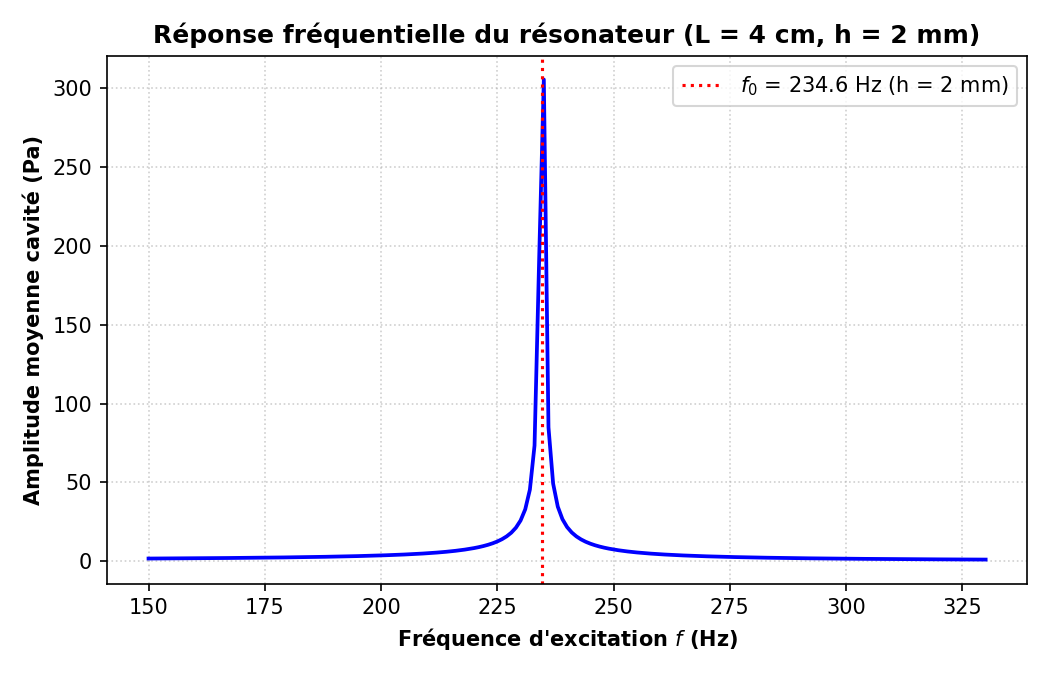
\includegraphics[width=0.48\textwidth]{doe_resonance.png}
\caption{Réponse fréquentielle de l'amplitude moyenne de cavité pour la géométrie de référence $L=4$ cm, \emph{sur la grille grossière} $h=2$ mm : le pic ($234{,}6$ Hz par interpolation parabolique, identique au Tableau \ref{tab:mesh_sensitivity}) donne $f_0$ de cette grille ; la valeur extrapolée au maillage nul vaut $221{,}0$ Hz (Tableau \ref{tab:gci}).}
\label{fig:freq_response}
\end{figure}

La Figure \ref{fig:freq_response} présente la courbe de réponse en amplitude pour $L=4\text{ cm}$, obtenue par balayage fréquentiel du solveur sur la grille $h=2$ mm. Le pic de résonance $f_0$ est extrait par interpolation parabolique autour du maximum. Précision importante pour la cohérence de l'article : chaque grille possède sa propre fréquence de pic (Tableau \ref{tab:mesh_sensitivity}) ; lorsque la suite du texte utilise une valeur de $f_0$, la grille correspondante est systématiquement indiquée.

\section{Identification de la Loi d'Échelle}
Le Tableau \ref{tab:f0_comparison} regroupe les fréquences de résonance propres $f_0(L)$ obtenues pour cinq longueurs de col.

\begin{table*}[t]
\centering
\caption{Confrontation des fréquences de résonance propres $f_0$ (Hz) pour cinq longueurs de col}
\label{tab:f0_comparison}
\begin{tabular}{c*{3}{>{\centering\arraybackslash}p{3cm}}}
\toprule
L (cm) & Théorie 1D ($\Delta L=0$) & FDM fin ($h=0{,}5$ mm) & FDM extrapolé ($h\to0$)\\
\midrule
2{,}0 & 341{,}2 & 297{,}0 & 292{,}2 \\
3{,}0 & 278{,}6 & 253{,}7 & 249{,}7 \\
4{,}0 & 241{,}3 & 224{,}8 & 221{,}0 \\
5{,}0 & 215{,}8 & 203{,}9 & 200{,}3 \\
6{,}0 & 197{,}0 & 188{,}0 & 184{,}9 \\
\bottomrule
\end{tabular}
\end{table*}

Pour identifier la loi d'échelle géométrique, nous confrontons \emph{à armes égales} deux modèles à deux paramètres, une loi de puissance empirique (A) et le modèle physique de Helmholtz à \emph{longueur effective} (B),
\begin{equation}
\underbrace{f_0(L) = A\, L^b}_{\text{(A) loi de puissance}}
\qquad
\underbrace{f_0(L) = \frac{A_H}{\sqrt{L + \Delta L_{\mathrm{eff}}}}}_{\text{(B) longueur effective}}
\end{equation}
Point méthodologique : les fréquences FDM portent une incertitude numérique d'environ $2\%$ (Section \ref{sec:convergence}), bien supérieure aux résidus d'ajustement. L'ajustement est donc réalisé sur les fréquences \emph{extrapolées de Richardson} (Tableau \ref{tab:f0_comparison}), \emph{pondéré} par les incertitudes GCI. Une précision s'impose sur le statut de cette pondération : le GCI est une \emph{borne prudente} de l'erreur de discrétisation, non un écart-type aléatoire gaussien, et les erreurs des différentes longueurs sont vraisemblablement \emph{corrélées} (même code, mêmes maillages, même extrapolation). Nous l'assimilons néanmoins à un $\sigma$ indicatif indépendant — hypothèse explicitement approximative — de sorte que le $\chi^2$ réduit, l'AICc et les intervalles de paramètres doivent se lire comme une \emph{analyse de sensibilité à intervalles numériques} plutôt que comme une inférence probabiliste stricte ; les $\chi^2/\mathrm{dof}$ très inférieurs à 1 reflètent d'ailleurs le conservatisme du GCI. La validation croisée \emph{leave-one-out} (LOO), indépendante de ce modèle d'erreur, complète la comparaison. Les résultats figurent dans le Tableau \ref{tab:model_selection}.

\begin{table*}[t]
\centering
\caption{Ajustement pondéré par l'incertitude numérique ($k=2$ paramètres ; $\chi^2$ réduit, AICc et erreur de prédiction leave-one-out)}
\label{tab:model_selection}
\begin{tabular}{>{\raggedright\arraybackslash}p{4.5cm}>{\centering\arraybackslash}p{5cm}>{\centering\arraybackslash}p{1.8cm}>{\centering\arraybackslash}p{1.6cm}>{\centering\arraybackslash}p{2.4cm}}
\toprule
Modèle & Paramètres ajustés & $\chi^2/\mathrm{dof}$ & AICc & LOO-RMSE (Hz) \\
\midrule
(A) Loi de puissance $A L^b$ & $A=57{,}4\pm4{,}5$, \; $b=-0{,}417\pm0{,}024$ & $0{,}09$ & $10{,}3$ & $2{,}93$ \\
(B) Longueur effective $A_H/\sqrt{L+\Delta L_{\mathrm{eff}}}$ & $A_H=47{,}7\pm1{,}4$, \; $\Delta L_{\mathrm{eff}}=6{,}6\pm2{,}3$ mm & $<0{,}01$ & $10{,}0$ & $\mathbf{0{,}51}$ \\
\bottomrule
\end{tabular}
\end{table*}

Une fois l'incertitude numérique propagée, les deux modèles sont \emph{compatibles} avec les données ($\chi^2/\mathrm{dof} < 1$) et l'écart $\Delta\text{AICc} = \text{AICc}_A - \text{AICc}_B \approx 0{,}3$ n'est \emph{pas décisif} : à ce niveau d'incertitude, les données seules ne permettent pas de trancher statistiquement entre les deux formes. Le modèle physique (B) reste néanmoins préféré pour trois raisons convergentes :
\begin{itemize}
    \item sa constante ajustée $A_H = 47{,}7 \pm 1{,}4$ est compatible avec la constante théorique \emph{a priori} $A_H^{\mathrm{th}} = 48{,}25$ ;
    \item sa longueur effective $\Delta L_{\mathrm{eff}} = 6{,}6\text{ mm} \approx 0{,}66\,R_{col}$ est du même ordre que la correction de bout de Rayleigh/Ingard \cite{ingard1953theory} ($0{,}6$–$0{,}85\,R_{col}$), \emph{à titre indicatif} — le modèle ne comportant pas de domaine de rayonnement extérieur (voir ci-dessous) ;
    \item sa capacité de prédiction hors échantillon est nettement supérieure (LOO-RMSE $0{,}5$ contre $2{,}9$ Hz).
\end{itemize}

L'exposant apparent $b \approx -0{,}42$ d'une loi de puissance n'est donc pas une physique alternative : une fonction en $1/\sqrt{L+\Delta L_{\mathrm{eff}}}$, observée sur une plage de $L$ restreinte, se confond localement avec une loi de puissance d'exposant intermédiaire. Enfin, $\Delta L_{\mathrm{eff}}$ est une correction \emph{effective} propre à la configuration numérique : elle agrège la transition col–cavité, la condition d'entrée de Dirichlet et la discrétisation en escalier, et ne constitue pas une vérification de la correction de bout de rayonnement au sens strict.

Pour dépasser la limite du faible échantillon, l'analyse est répétée sur un jeu élargi de douze longueurs de col ($1{,}5$ à $7{,}0$ cm). La tendance se renforce : $\Delta\text{AICc}$ passe de $0{,}3$ à $\approx 1{,}8$ en faveur du modèle de longueur effective, dont les paramètres restent stables ($A_H = 48{,}6 \approx A_H^{\mathrm{th}}$, $\Delta L_{\mathrm{eff}} = 0{,}68\,R_{col}$) et la prédiction hors échantillon très supérieure (LOO-RMSE $0{,}3$ contre $3{,}3$ Hz). L'écart demeure toutefois en deçà du seuil d'exclusion forte ($\Delta\text{AICc}>10$) : le modèle physique est \emph{favorisé}, sans être formellement le seul admissible.

\subsection{Décomposition intérieure/extérieure par condition d'impédance de rayonnement}
\label{sec:radiation}
Pour séparer la part intérieure de $\Delta L_{\mathrm{eff}}$ de la charge de rayonnement extérieure, une seconde configuration est construite : l'embouchure ($z=0$, $r\leq R_{col}$) n'est plus une frontière de Dirichlet mais porte l'impédance de rayonnement d'un piston bafflé en basse fréquence \cite{rayleigh1896, morse1968theoretical},
\begin{equation}
Z_{\mathrm{rad}} = \rho c\left[\tfrac{1}{2}(kR_{col})^2 + i\,\tfrac{8}{3\pi}\,kR_{col}\right],
\end{equation}
imposée par une condition de Robin ($\partial p/\partial z = i\omega\rho\, p/Z_{\mathrm{rad}}$, nœud fantôme), l'excitation devenant un forçage volumique dans la cavité. La partie imaginaire de $Z_{\mathrm{rad}}$ encode analytiquement la correction extérieure $\Delta L_{\mathrm{ext}} = 8R_{col}/(3\pi) \approx 0{,}849\,R_{col}$ ; sa partie réelle introduit l'amortissement par rayonnement.

Les deux configurations sont résolues sur la \emph{même} grille ($h=1$ mm) pour cinq longueurs, de sorte que le biais de discrétisation s'annule au premier ordre dans la différence. L'ajustement donne $\Delta L_{\mathrm{Dirichlet}} = 0{,}675\,R_{col}$ et $\Delta L_{\mathrm{rayonnement}} = 1{,}499\,R_{col}$, soit un décalage de $0{,}825\,R_{col}$, en accord à $2{,}8\%$ avec la valeur analytique $8/(3\pi) = 0{,}849$. Ce résultat est \emph{cohérent} avec la décomposition additive $\Delta L_{\mathrm{tot}} = \Delta L_{\mathrm{int}} + \Delta L_{\mathrm{ext}}$ ; il identifie du même coup $\Delta L_{\mathrm{int}} \approx 0{,}68\,R_{col}$ comme la correction propre à la jonction col–cavité. Précisons honnêtement sa portée : la réactance imposée \emph{contenant} $8R_{col}/(3\pi)$, ce test montre essentiellement que la condition de Robin est correctement implémentée et que la chaîne calcul–extraction–régression restitue la variation imposée — c'est une vérification de cohérence, non un calcul \emph{ab initio} du rayonnement, qui exigerait un domaine extérieur maillé avec condition de Sommerfeld ou couche parfaitement adaptée (PML) \cite{berenger1994perfectly}. Le facteur de qualité de rayonnement mesuré sur ces réponses ($Q_{\mathrm{rad}} \approx 150$–$320$, croissant quand $f_0$ diminue) confirme par ailleurs que le rayonnement est un canal de pertes secondaire devant les pertes viscothermiques ($Q_{\mathrm{visc}}\approx47$, Section \ref{sec:losses}).

\begin{figure*}[ht]
\centering
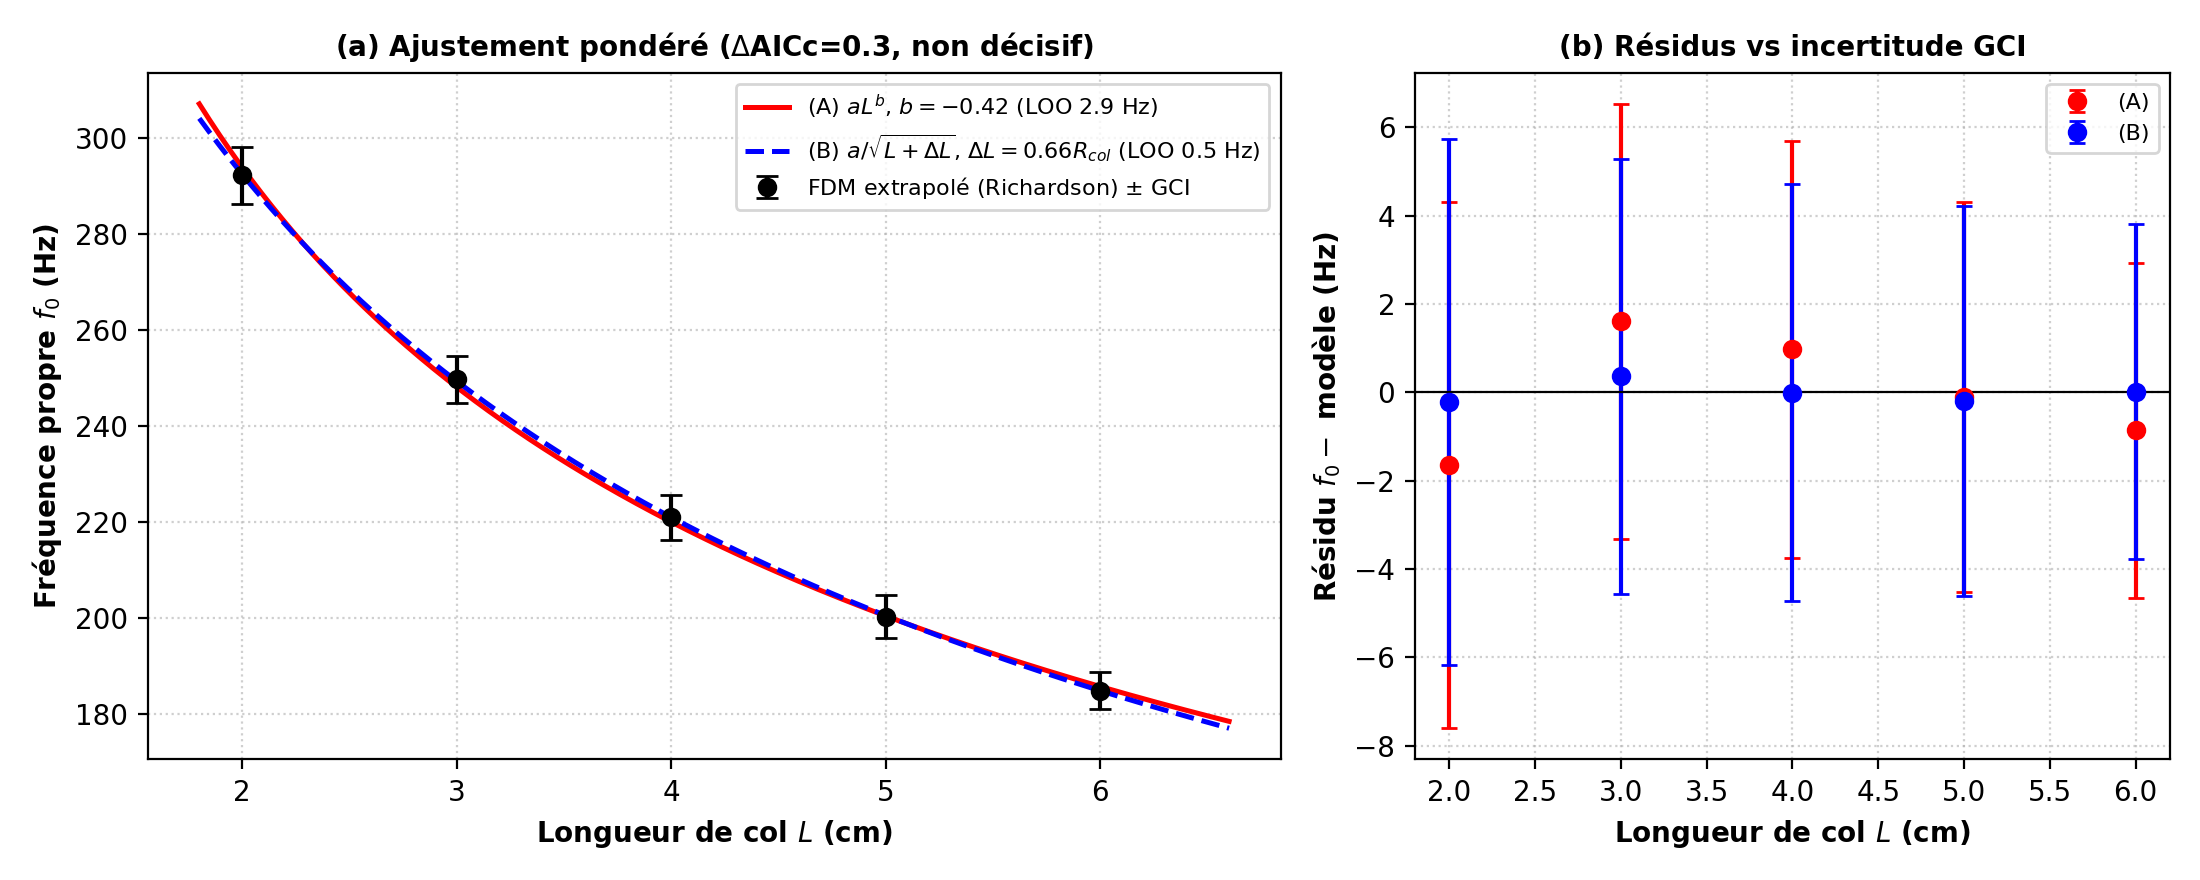
\includegraphics[width=0.95\textwidth]{scaling_law_gci.png}
\caption{(a) Ajustement pondéré par l'incertitude numérique : fréquences extrapolées de Richardson avec barres d'incertitude GCI ($\approx 2\%$), modèle de longueur effective (bleu) et loi de puissance (rouge). Les deux modèles restent dans les barres d'erreur ($\Delta$AICc non décisif) ; la longueur effective prédit toutefois nettement mieux hors échantillon (LOO). (b) Résidus des deux modèles rapportés à l'incertitude GCI.}
\label{fig:scaling_gci}
\end{figure*}

La Figure \ref{fig:scaling_gci}(a) illustre ces ajustements. Les limites scientifiques majeures de cette étude restent le faible nombre de géométries testées (cinq longueurs), l'incertitude numérique résiduelle ($\approx 2\%$, cf. Section \ref{sec:convergence}), la géométrie en escalier au raccordement col–cavité, et l'absence de confrontation expérimentale directe.

\section{Pertes Viscothermiques et Facteur de Qualité}
\label{sec:losses}
Le solveur fréquentiel précédent est sans perte : sa résonance n'est pas amortie (la largeur apparente de la Figure \ref{fig:freq_response} n'est due qu'à la résolution finie du balayage). Pour introduire un amortissement, nous résolvons l'équation d'onde \emph{amortie} en régime transitoire par un schéma leapfrog explicite,
\begin{equation}
\frac{\partial^2 p}{\partial t^2} + \gamma(r,z)\frac{\partial p}{\partial t} = c^2\!\left(\frac{\partial^2 p}{\partial r^2} + \frac{1}{r}\frac{\partial p}{\partial r} + \frac{\partial^2 p}{\partial z^2}\right),
\end{equation}
en confrontant deux mécanismes de dissipation.

\subsection{Pertes volumiques (Stokes) : négligeables}
L'absorption classique de l'air (viscosités de cisaillement et de volume, conduction thermique) donne le coefficient d'atténuation de Stokes $\alpha = \delta_{\mathrm{diff}}\,\omega^2/(2c^3)$ \cite{stokes1845theories}, soit un amortissement uniforme $\gamma_{\mathrm{bulk}} = \delta_{\mathrm{diff}}\,\omega^2/c^2$. Avec une diffusivité du son $\delta_{\mathrm{diff}}\approx 3{,}8\times10^{-5}\text{ m}^2/\text{s}$, le facteur de qualité associé atteint $Q_{\mathrm{bulk}}\approx 2\times10^{6}$ : aux échelles centimétriques, ce mécanisme est totalement négligeable.

\subsection{Pertes viscothermiques de couche limite : dominantes}
Le mécanisme réel est la friction visqueuse et la conduction thermique dans la fine couche limite acoustique sur les parois du \emph{col}, où la vitesse particulaire est maximale \cite{crandall1926theory, morse1968theoretical}. Un bilan d'énergie (énergie du mode rapportée à la puissance dissipée sur la paroi du col, de résistance de surface $R_s=\sqrt{\rho\mu\omega/2}\,[1+(\gamma-1)/\sqrt{Pr}]$) conduit au facteur de qualité analytique
\begin{equation}
\label{eq:Qvisc}
Q_{\mathrm{visc}} = \frac{R_{col}}{F_t\,\delta_v}, \quad \delta_v=\sqrt{\frac{2\mu}{\rho\,\omega_0}}, \quad F_t = 1+\frac{\gamma-1}{\sqrt{Pr}}\approx 1{,}48,
\end{equation}
où $\delta_v$ est l'épaisseur de couche limite visqueuse. L'étude transitoire est menée sur la grille $h=2$ mm, dont la fréquence propre vaut $f_0 = 234{,}6\text{ Hz}$ (Tableau \ref{tab:mesh_sensitivity}) : c'est cette valeur — et non la valeur extrapolée $221{,}0$ Hz — qui fixe l'excitation et $\delta_v\approx0{,}14\text{ mm}$, d'où $Q_{\mathrm{visc}}\approx47$. L'écart de $6\%$ entre les deux fréquences ne modifierait $Q_{\mathrm{visc}}$ que d'environ $3\%$ ($Q\propto\sqrt{f_0}$), sans incidence sur les conclusions. La valeur obtenue est cohérente avec les mesures sur résonateurs réels (Section suivante).

Le solveur transitoire n'implémente pas cette couche limite sub-millimétrique (qui exigerait $h<0{,}1\text{ mm}$) : il utilise un \emph{modèle réduit d'amortissement équivalent}, un terme $\gamma$ localisé dans le col dont l'amplitude est \emph{calibrée} pour que le facteur de qualité de la décroissance libre reproduise $Q_{\mathrm{visc}}$. L'accord obtenu ($Q=47{,}5$, écart $0{,}1\%$) n'est donc pas une validation indépendante mais un simple \emph{contrôle de cohérence} de cette calibration ; de même, la carte de dissipation (Figure \ref{fig:losses}c) reflète la localisation \emph{imposée} de $\gamma$, non une émergence spontanée. Ce modèle réduit sert uniquement à \emph{illustrer} qualitativement les signatures de l'amortissement : décroissance impulsionnelle, chute exponentielle de l'énergie acoustique totale (d'où l'extraction de $Q$) et concentration de la dissipation dans le col (Figure \ref{fig:losses}).

\begin{figure*}[t]
\centering
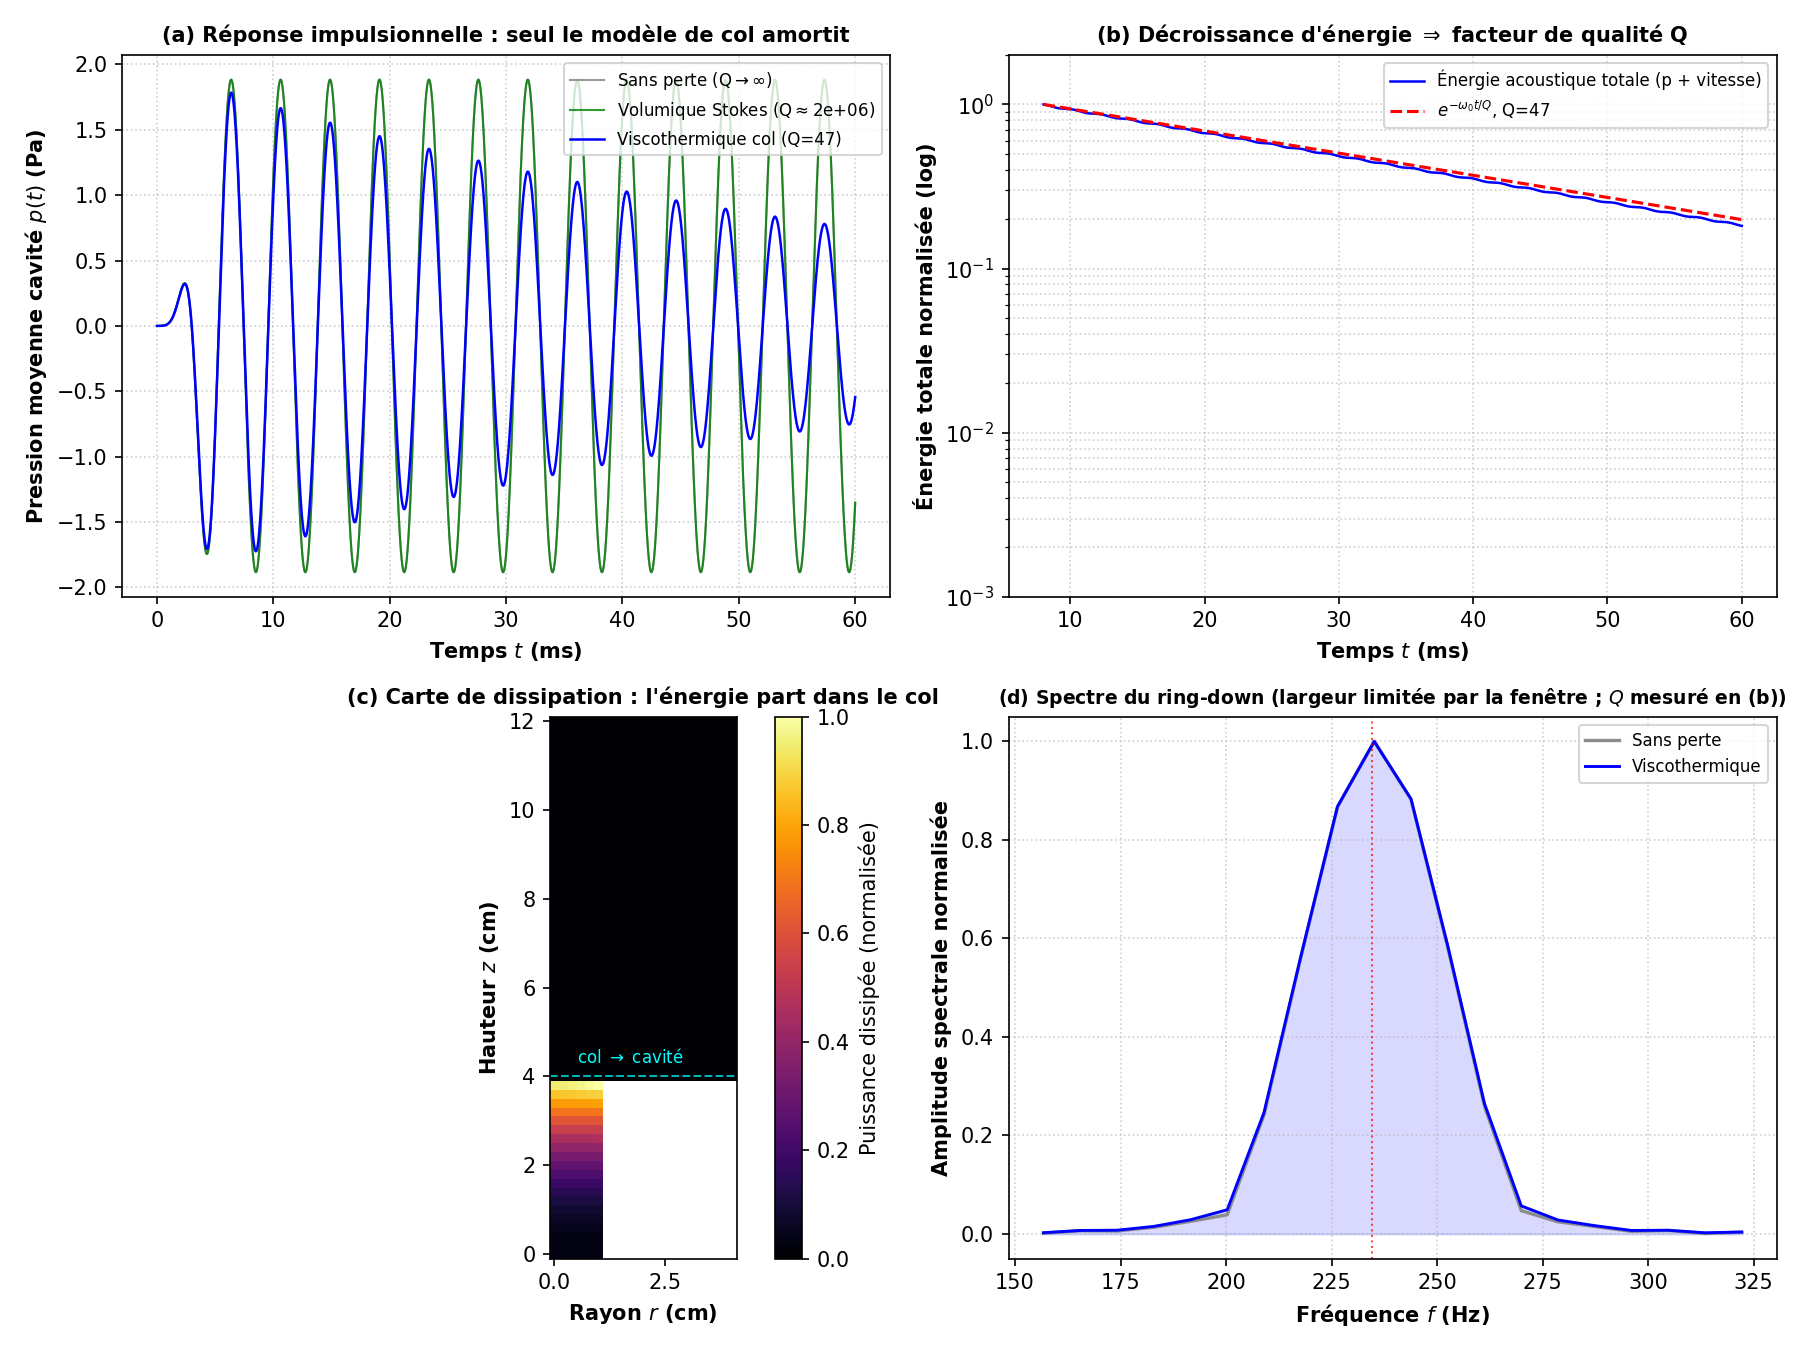
\includegraphics[width=0.92\textwidth]{phase1_losses.png}
\caption{Pertes du résonateur ($L=4$ cm), modèle réduit d'amortissement équivalent calibré. (a) Réponse impulsionnelle : seul le modèle viscothermique du col amortit ; le modèle volumique est indiscernable du cas sans perte. (b) Décroissance de l'énergie acoustique totale (potentielle en $p^2$ et cinétique en $|\mathbf{u}|^2$) en échelle logarithmique, d'où $Q$. (c) Carte de dissipation, reflétant la localisation imposée de l'amortissement dans le col. (d) Spectre du ring-down : la largeur visible est dominée par la fenêtre d'observation finie ($\approx 4/T$) et ne résout pas l'élargissement physique $\Delta f=f_0/Q\approx5$ Hz ; le facteur de qualité est mesuré en domaine temporel (panneau b).}
\label{fig:losses}
\end{figure*}

\subsection{Confrontation à la littérature}
Pour les cinq géométries, la fréquence propre FDM tombe dans la bande de correction de bout $\Delta L\in[0{,}60;0{,}85]\,R_{col}$ d'Ingard \cite{ingard1953theory} (Figure \ref{fig:verif}a). Le facteur de qualité $Q\approx47$ est compatible avec les valeurs mesurées sur des résonateurs réels ($Q\sim30$–$70$, Moloney \cite{moloney2004quality}), et la loi d'échelle $Q_{\mathrm{visc}}\propto\sqrt{\omega_0}$ reproduit la tendance attendue : les résonateurs plus aigus sont moins amortis (Figure \ref{fig:verif}b).

\begin{figure*}[t]
\centering
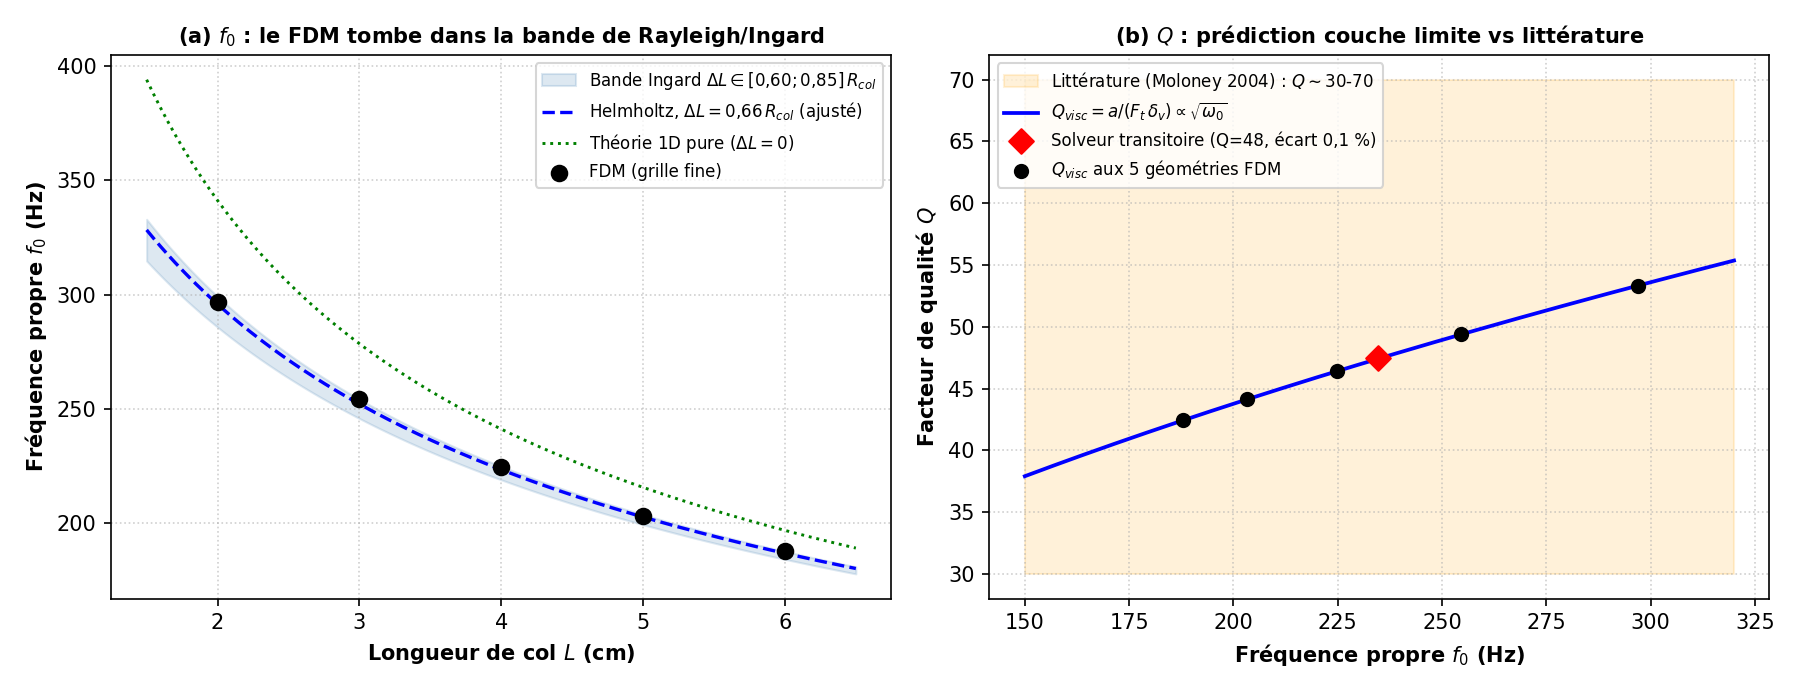
\includegraphics[width=0.92\textwidth]{phase2_verification.png}
\caption{Comparaison avec les corrections de longueur et facteurs de qualité de la littérature. (a) Les fréquences FDM tombent dans la bande de Rayleigh/Ingard et loin de la théorie 1D pure — cohérence, et non vérification indépendante. (b) Le facteur de qualité viscothermique $Q=R_{col}/(F_t\delta_v)$ suit la loi en $\sqrt{\omega_0}$ ; le point du solveur transitoire et la plage de la littérature (Moloney 2004) sont indiqués.}
\label{fig:verif}
\end{figure*}

\section{Détails Numériques et Reproductibilité}
\label{sec:repro}
Pour la reproductibilité, les paramètres numériques sont les suivants. Le système linéaire creux (format CSR, assemblage COO) est résolu par factorisation LU directe (\texttt{scipy.sparse.linalg.spsolve}, SuperLU), en double précision complexe. La fréquence propre est extraite par un balayage grossier (pas de $2$ Hz) suivi d'un balayage fin (pas de $0{,}25$–$0{,}3$ Hz sur $\pm2{,}5$ Hz autour du maximum) et d'une interpolation parabolique à trois points ; la stabilité de $f_0$ vis-à-vis du pas de balayage est vérifiée par un test automatique (variation $<0{,}5$ Hz entre pas de $1$ et $0{,}5$ Hz). Le solveur transitoire utilise un schéma leapfrog explicite avec $\Delta t = 0{,}85\,h/(c\sqrt{2})$ (soit $\mathrm{CFL}_{2D}=0{,}85$ ; $\Delta t \approx 3{,}5\ \mu$s à $h=2$ mm) sur une durée de $60$ ms. Les calculs sont exécutés sur un ordinateur portable x86-64 (CPU seul, un cœur) en Python/NumPy/SciPy ; l'intégralité du code, des données et des figures est régénérable par un script unique (\texttt{run\_all.py}), accompagné de tests automatiques (symétrie d'axe, plage de résonance, décroissance de $f_0$ avec $L$, stabilité au pas fréquentiel, ordre MMS).

\section{Limites et Conclusion}
Le solveur FDM axisymétrique développé reproduit la décroissance attendue de la fréquence de résonance avec la longueur du col. La démarche de vérification et validation est complète et hiérarchisée : le \emph{code} est vérifié par solution manufacturée (ordre $2{,}03$) ; la \emph{solution} l'est par une étude GCI sur trois grilles, complétée d'une quatrième grille de contrôle qui confirme la stabilité de l'ordre observé ($\approx 0{,}9$–$1{,}1$) et des extrapolations de Richardson ($0{,}01$–$0{,}32\%$ d'écart entre triplets) ; le \emph{modèle} fait l'objet d'une première validation sur deux configurations expérimentales publiées (écarts de $0{,}6\%$ et $2{,}2\%$, sans paramètre ajusté). Une fois l'incertitude numérique ($\approx2\%$) propagée dans l'ajustement pondéré — traité en analyse de sensibilité, le GCI n'étant pas un écart-type statistique —, la loi de puissance et le modèle à longueur effective sont \emph{indiscernables} ($\Delta\text{AICc}$ non décisif, de $0{,}3$ à $1{,}8$ selon l'échantillon) ; le modèle physique est toutefois préféré car sa constante ($A_H\approx A_H^{\mathrm{th}}$), sa longueur effective ($\Delta L_{\mathrm{eff}} \approx 0{,}66$–$0{,}68\,R_{col}$, du même ordre que la correction de Rayleigh/Ingard) et sa prédiction hors échantillon sont nettement meilleures. Ces résultats sont \emph{compatibles} avec la théorie classique dans les limites de l'incertitude numérique, sans en constituer une vérification stricte : $\Delta L_{\mathrm{eff}}$ reste une correction effective, et l'exposant apparent $b \approx -0{,}42$ un artefact d'une plage géométrique restreinte. La configuration à impédance de rayonnement (Section \ref{sec:radiation}) sépare la part intérieure ($0{,}68\,R_{col}$, jonction col–cavité) de la charge extérieure, le décalage mesuré ($0{,}825\,R_{col}$) restituant à $2{,}8\%$ la réactance de piston bafflé imposée — test de cohérence de la chaîne complète, à distinguer d'un calcul \emph{ab initio} du rayonnement. Un modèle réduit d'amortissement équivalent, calibré sur une estimation viscothermique ($Q\approx47$, compatible avec la littérature), illustre les signatures des pertes sans les résoudre. Un domaine extérieur maillé (Sommerfeld ou PML \cite{berenger1994perfectly}), une validation élargie (plusieurs rapports col/cavité, réponse complète) et une campagne expérimentale propre (protocole fourni avec le dépôt) constituent les prochaines étapes naturelles.

\bibliographystyle{plain}
\bibliography{references}

\end{document}
